\documentclass{beamer}

\mode<presentation> {
%\usetheme{AnnArbor}
%\usetheme{Antibes}
%\usetheme{Bergen}
%\usetheme{Berkeley}
%\usetheme{Berlin}
%\usetheme{Boadilla}
%\usetheme{CambridgeUS}
%\usetheme{Copenhagen}
%\usetheme{Darmstadt}
%\usetheme{Dresden}
%\usetheme{Frankfurt}
%\usetheme{Goettingen}
%\usetheme{Hannover}
%\usetheme{Ilmenau}
%\usetheme{JuanLesPins}
%\usetheme{Luebeck}
\usetheme{Madrid}
%\usetheme{Malmoe}
%\usetheme{Marburg}
%\usetheme{Montpellier}
%\usetheme{PaloAlto}
%\usetheme{Pittsburgh}
%\usetheme{Rochester}
%\usetheme{Singapore}
%\usetheme{Szeged}
%\usetheme{Warsaw}

%\usecolortheme{albatross}
\usecolortheme{beaver}
%\usecolortheme{beetle}
%\usecolortheme{crane}
%\usecolortheme{dolphin}
%\usecolortheme{dove}
%\usecolortheme{fly}
%\usecolortheme{lily}
%\usecolortheme{orchid}
%\usecolortheme{rose}
%\usecolortheme{seagull}
%\usecolortheme{seahorse}
%\usecolortheme{whale}
%\usecolortheme{wolverine}
%\setbeamertemplate{footline}
%{
%	\leavevmode%
%	\hbox{%
%		\begin{beamercolorbox}[wd=.333333\paperwidth,ht=2.25ex,dp=1ex,center]{author in head/foot}%
%			\usebeamerfont{author in head/foot}\insertshortauthor
%		\end{beamercolorbox}%
%		\begin{beamercolorbox}[wd=.46\paperwidth,ht=2.25ex,dp=1ex,center]{title in head/foot}%
%			\usebeamerfont{title in head/foot}\insertshorttitle
%		\end{beamercolorbox}%
%		\begin{beamercolorbox}[wd=.2\paperwidth,ht=2.25ex,dp=1ex,right]{date in head/foot}%
%			\usebeamerfont{date in head/foot}
%			\insertframenumber{}% / \inserttotalframenumber
%			\hspace*{2ex} 
%	\end{beamercolorbox}}%
%	\vskip0pt%
%}
}

\usepackage{graphicx} % Allows including images
\usepackage{booktabs} % Allows the use of \toprule, \midrule and \bottomrule in tables
\usepackage{amsmath}
\usepackage{amsfonts}
\usepackage{ifthen}
\usepackage{amssymb}
\usepackage{amsbsy}
\usepackage{bm}
\usepackage{ulem}
\usepackage{float}
\usepackage{latexsym}
\usepackage{comment}
\usepackage{graphicx}
\usepackage{amstext}
\usepackage{latexsym}
\usepackage{arydshln}
\usepackage{longtable}
\usepackage{enumerate}
\usepackage{multirow}
\usepackage{cases}
\usepackage{geometry}
\usepackage{mathtools}
\usepackage{subeqnarray}
\usepackage{textcomp}
\usepackage{hyperref}
%\usepackage{subfigure}
\usepackage{url}
\usepackage{threeparttable}
\usepackage{xr}
\usepackage{multirow}
\usepackage{wrapfig}
\usepackage{lscape}
\usepackage{rotating}
\usepackage{subcaption}
\usepackage{epstopdf}
\usepackage{verbatim}
\usepackage{xcolor}
\usepackage[sort&compress]{natbib}
\usepackage{bm}


\newcommand{\bA}{\mathbf{A}}
\newcommand{\bB}{\mathbf{B}}
\newcommand{\bD}{\mathbf{D}}
\newcommand{\bF}{\mathbf{F}}
\newcommand{\bI}{\mathbf{I}}
\newcommand{\bLambda}{{\bm\Lambda}}
\newcommand{\bOmega}{{\bm\Omega}}
\newcommand{\bM}{\mathbf{M}}
\newcommand{\bN}{\mathbf{N}}
\newcommand{\bphi}{{\bm\phi}}
\newcommand{\bpsi}{{\bm\psi}}
\newcommand{\brho}{{\bm\rho}}
\newcommand{\bvarphi}{{\bm\varphi}}
\newcommand{\bW}{\mathbf{W}}
\newcommand{\sT}{\mathrm{T}}
\newcommand{\bZ}{\mathbf{Z}}
\newcommand{\shalf}{\mbox{{\footnotesize$\frac{1}{2}$}}}



\setbeamertemplate{theorems}[numbered]
\newtheorem{prop}{Proposition}
\let\oldframe\frame
\renewcommand{\frame}{%
\oldframe
\let\olditemize\itemize
\renewcommand\itemize{\olditemize\addtolength{\itemsep}{10pt}}%
}



%----------------------------------------------------------------------------------------
%	TITLE PAGE
%----------------------------------------------------------------------------------------


\title[Hierarchical Spatial FW Model for MET]{A Hierarchical Spatial Finlay-Wilkinson Model for Multi-Environment Trial Analysis}

\author[Guo, X., Dutta, S., Nettleton, D.]{Xingche Guo, Somak Dutta, Dan Nettleton}
\institute[ISU]{Dept. of Statistics, Iowa State University}
\date[JSM, 2019]{Joint Statistical Meetings, 2019}

\AtBeginSection[]{
	\begin{frame}
		\vfill
		\centering
		\begin{beamercolorbox}[sep=8pt,center,shadow=true,rounded=true]{title}
			\usebeamerfont{title}\insertsectionhead\par%
		\end{beamercolorbox}
		\vfill
	\end{frame}
}





\begin{document}
\begin{frame}
\titlepage
\end{frame}

%\begin{frame}
%	\frametitle{Overview}
%	\tableofcontents
%\end{frame}


\begin{frame}
	\frametitle{Finlay-Wilkinson (FW) model}
	\begin{itemize}
	\item FW model: 
	$$y_{ijk} = \mu + g_i + h_j + b_i h_j + e_{ijk},$$
	\item A model for characterizing genotype-by-environment interaction.
 \item For genotype $i$:
 $$y_{ijk} = (\mu + g_i) +  (b_i + 1) h_j + e_{ijk},$$
 FW model becomes a linear model with intercept $\mu + g_i$ and slope $b_i + 1 $.
	\end{itemize}		
\end{frame}



\begin{frame}
\frametitle{Finlay-Wilkinson (FW) model}
This plot gives one example of the fitted FW model (using G2F data). Each line represents the linear relationship between grain yield and location effect for one genotype.
	\begin{figure}[H]
		\centering
		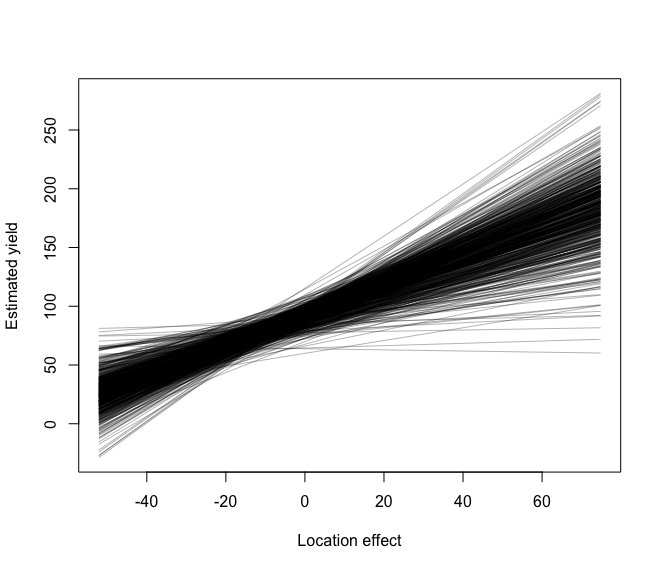
\includegraphics[width = 0.65\textwidth]{image8.png}
	\end{figure}
\end{frame}




\begin{frame}
	\frametitle{Residuals of FW model for two fields}
	\textbf{Problem:} the residuals are highly spatially correlated.
	\begin{figure}[H]
		\centering
		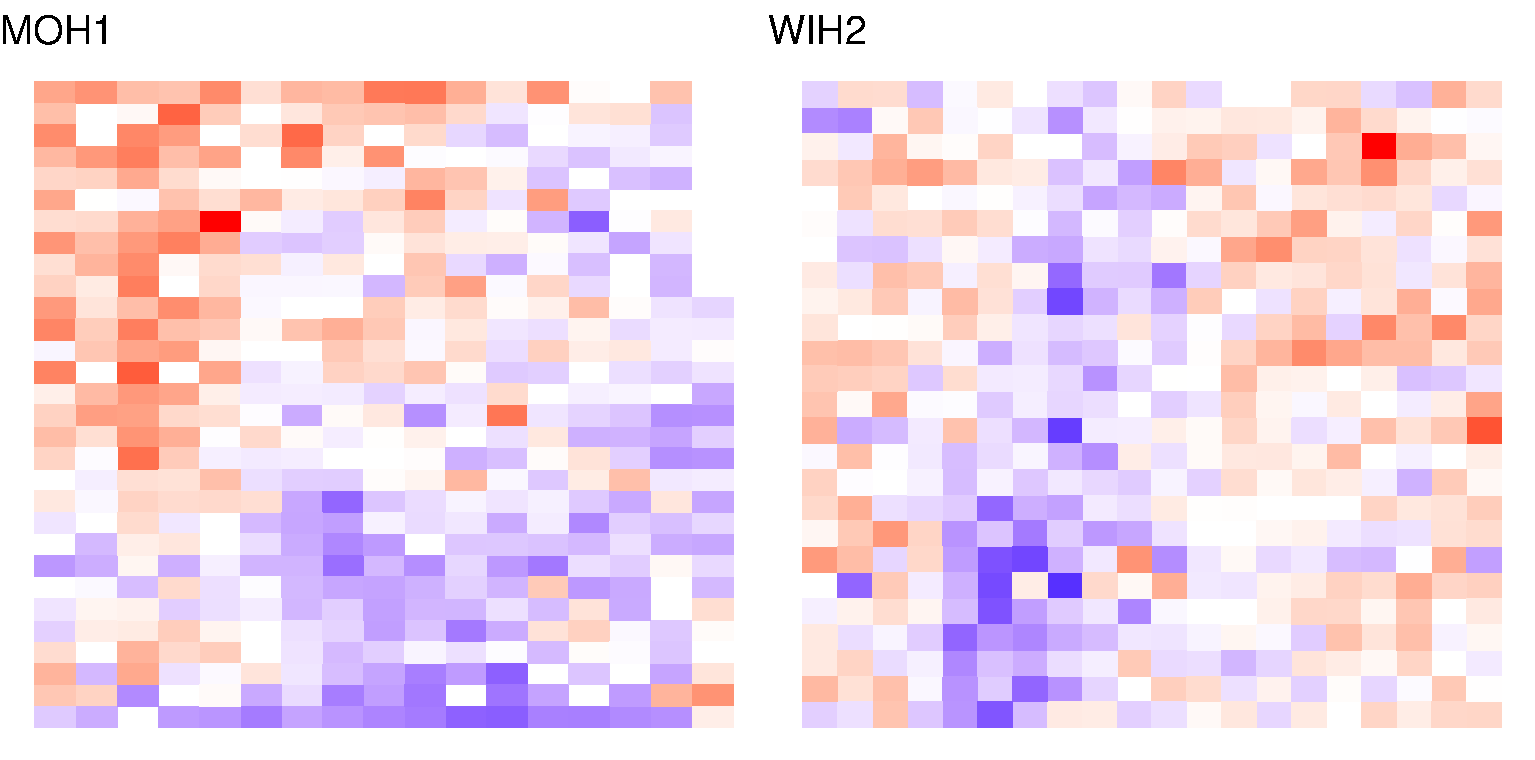
\includegraphics[width = 0.91\textwidth]{resid_plot_2.pdf}
	\end{figure}
\end{frame}



\begin{frame}
	\frametitle{Hierarchical spatial Finlay-Wilkinson (SFW) model}
	\begin{itemize}
	\item Data model:
\begin{equation*}
[y_{ijk} | \mu, \mathbf{g}, \mathbf{b}, \mathbf{h}, \bphi ] \ \ \overset{indep}{\sim} \ \  \mathcal{N}(\mu + g_i + h_j + b_i h_j + \phi_{ijk}, \sigma_e^2),
\end{equation*}

	\item Prior distributions for genotype, slope, and field effects:
	$$  [\mathbf{g}] \sim \mathcal{N}(\bm{0}, \bA \sigma_g^2); \ \ \ \ [\mathbf{b}] \sim \mathcal{N}(\bm{0}, \bA \sigma_b^2); $$
        $$[\mathbf{h}|\bm{\gamma}] \sim \mathrm{N}( \gamma_1 \bZ_1 + \dots + \gamma_l \bZ_l + \dots + \gamma_L \bZ_L
         , \mathbf{I} \sigma_h^2)$$
	\end{itemize}
	$\bA$ is a known matrix describing the correlation structure of $\mathbf{g}$ and $\mathbf{b}$, $\bZ_{l}$ is the $l$th environment-specific covariate.
\end{frame}


\begin{frame}
	\frametitle{Prior distributions for spatial effects}
	\begin{itemize}
	\item A popular model for fertility adjustment in agricultural field trials is the \textbf{first order intrinsic autoregression} \citep{besag1999bayesian,dutt:mond:2015}.

\item First order Intrinsic Autoregressive prior (Besag 1995, Besag 1999):

\begin{equation*}
[\bpsi_j|\theta_j,\sigma^2_j] \propto |\sigma^{-2}_j\bW_j|_+^{1/2}\exp\left( -\shalf\sigma^{-2}_j\bpsi_j\bW_j\bpsi_j\right)
\end{equation*}
where
\[\bpsi_j\bW_j\bpsi_j = \theta_j\sum\sum(\psi_{u,v} - \psi_{u-1,v})^2 + {\bar\theta}_j\sum\sum(\psi_{u,v} - \psi_{u,v-1})^2\]

\item  The distribution of $\pmb{\psi}_j$ is \textbf{invariant} to the addition of arbitrary constant.

	\end{itemize}

\end{frame}




\begin{frame}
	\frametitle{Prior distributions for spatial effects}
	\begin{itemize}

\item The intrinsic model has an indeterminate overall level.
\item The overall levels of the field specific spatial effects are completely confounded with the location effects.
\item Not directly applicable for yield prediction.
\item  \textbf{A hard constraint}:  set the average of the spatial effects to zero.
\end{itemize}
 
\end{frame}



\begin{frame}
	\frametitle{Projected intrinsic autoregression (PIAR) prior}

Special structure of $\bW_j$:

  	\begin{itemize}
         \item Then the spectral decomposition of $\bW_j$ is given by 
         $$\bM_j\bW_j\bM_j^\sT = \theta_j\bLambda_{r_j}\otimes\mathbf{I}_{c_j} + \bar\theta_j\mathbf{I}_{r_j}\otimes\bLambda_{c_j}.$$
         \item where $\bM_j = \bN_{r_j}\otimes\bN_{c_j}$.
         \item $\bLambda_k$ denote the $k\times k$ diagonal matrix  whose $u$th diagonal entry is $4\sin^2\{\pi(u-1)/(2k)\}.$
	\item $\bN_k$ denotes the $k\times k$ orthogonal matrix whose $(u,v)$th entry is $1/\sqrt{k}$ if $u=1,$ $\forall v,$ and $(2/k)^{1/2}\cos\{\pi(u-1)(v-1/2)/k\}$ otherwise.
	\end{itemize}
	
\end{frame}


\begin{frame}
	\frametitle{Projected intrinsic autoregression (PIAR) prior}

  	\begin{itemize}
	\item The Gaussian projected intrinsic autoregression (PIAR) on the $r_j \times c_j$ regular array is then defined as:
	\begin{equation*}
\bphi_j = \bB_j \bvarphi_j,\qquad \bvarphi_j\sim{\mathcal N}(\mathbf{0},\bD_j^{-1}),
\end{equation*}
\item  $\bB_{j}^{\sT}$ denotes the $(r_jc_j-1)\times r_jc_j$ matrix consisting of last $r_jc_j-1$ rows of $\bM_j$.
\item $\bD_j$ denotes the diagonal matrix consisting of the nonzero eigenvalues of $\bW_j$.
	\end{itemize}
	
\end{frame}




\begin{frame}
	\frametitle{Matrix free computation}
	
	\begin{itemize}
	\item  The covariance matrix of the Gaussian PIAR is a dense singular matrix.
	\item The computation load for generating $\bphi_j$ from PIAR using knowledge of multivariate statistics is ${\mathcal O}((r_jc_j)^3/3)$.
	\item Assume small number of missing plots (denote $M_j$ as the number of missing plots).
)
	\item Thus matrix-vector multiplications with $\bB_j$ and $\bB^{\sT}_j$ can also be performed using these discrete cosine transformations (DCT).
	\item The computation load of matrix free computation algorithm is $\mathcal{O}( r_j c_j M_j \log r_jc_j +  M_j^3/3)$.	\end{itemize}
	
\end{frame}





\begin{frame}
	\frametitle{Within-fields prediction}
	
	\begin{itemize}
	\item Given grain yields values for some plots in fields, predict the yields for the rest plots.
	\item Implement posterior predictive distributions.
	\item Important to account for the spatial correlation between plots.
	\item Kinship information plays a decisive role when there are new crop varieties in the testing sets.
	\end{itemize}
	
\end{frame}



\begin{frame}
	\frametitle{Within-fields prediction}
	50 Plot Yield Prediction Intervals ($95\%$ Credible Level).
	\begin{figure}[H]
		\centering
		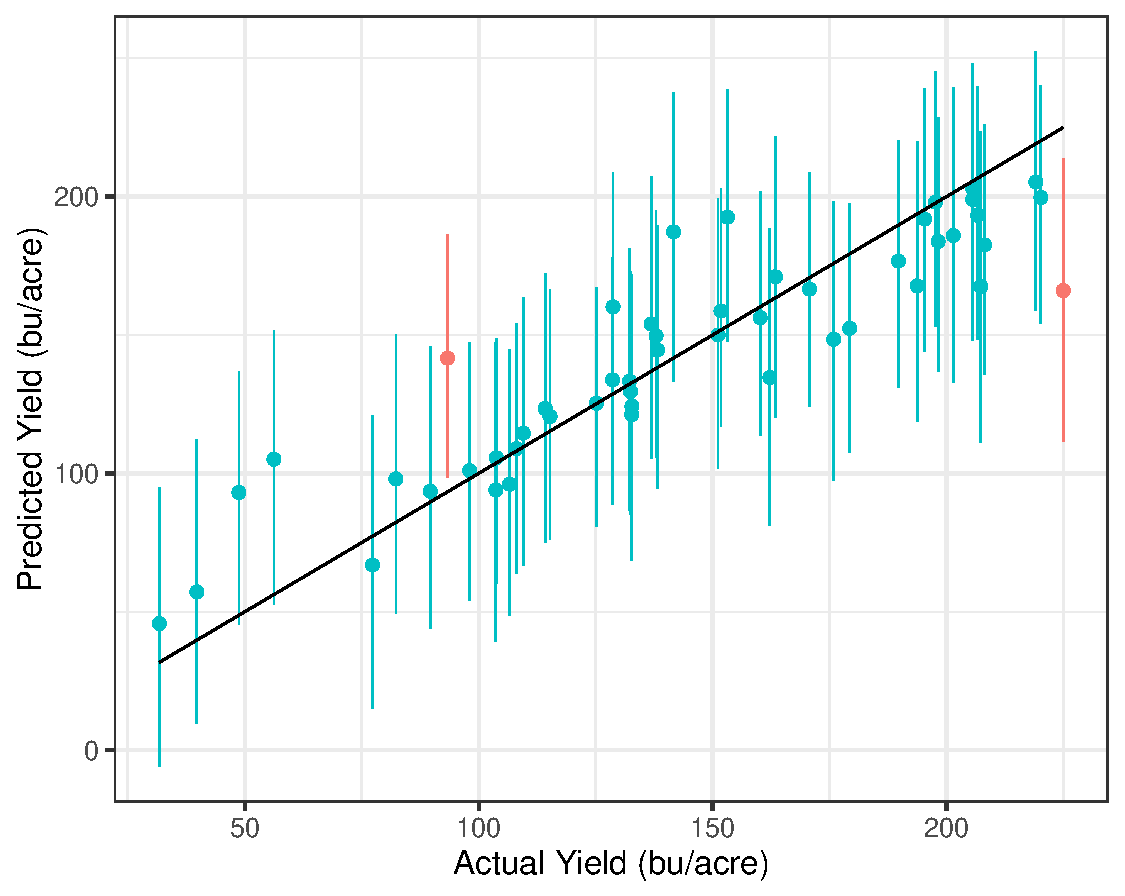
\includegraphics[width = 0.75\textwidth]{true_vs_predint.pdf}
	\end{figure}
\end{frame}



\begin{frame}
	\frametitle{Within-fields prediction}
	Reduced error for yield prediction.
	\begin{figure}[H]
		\centering
		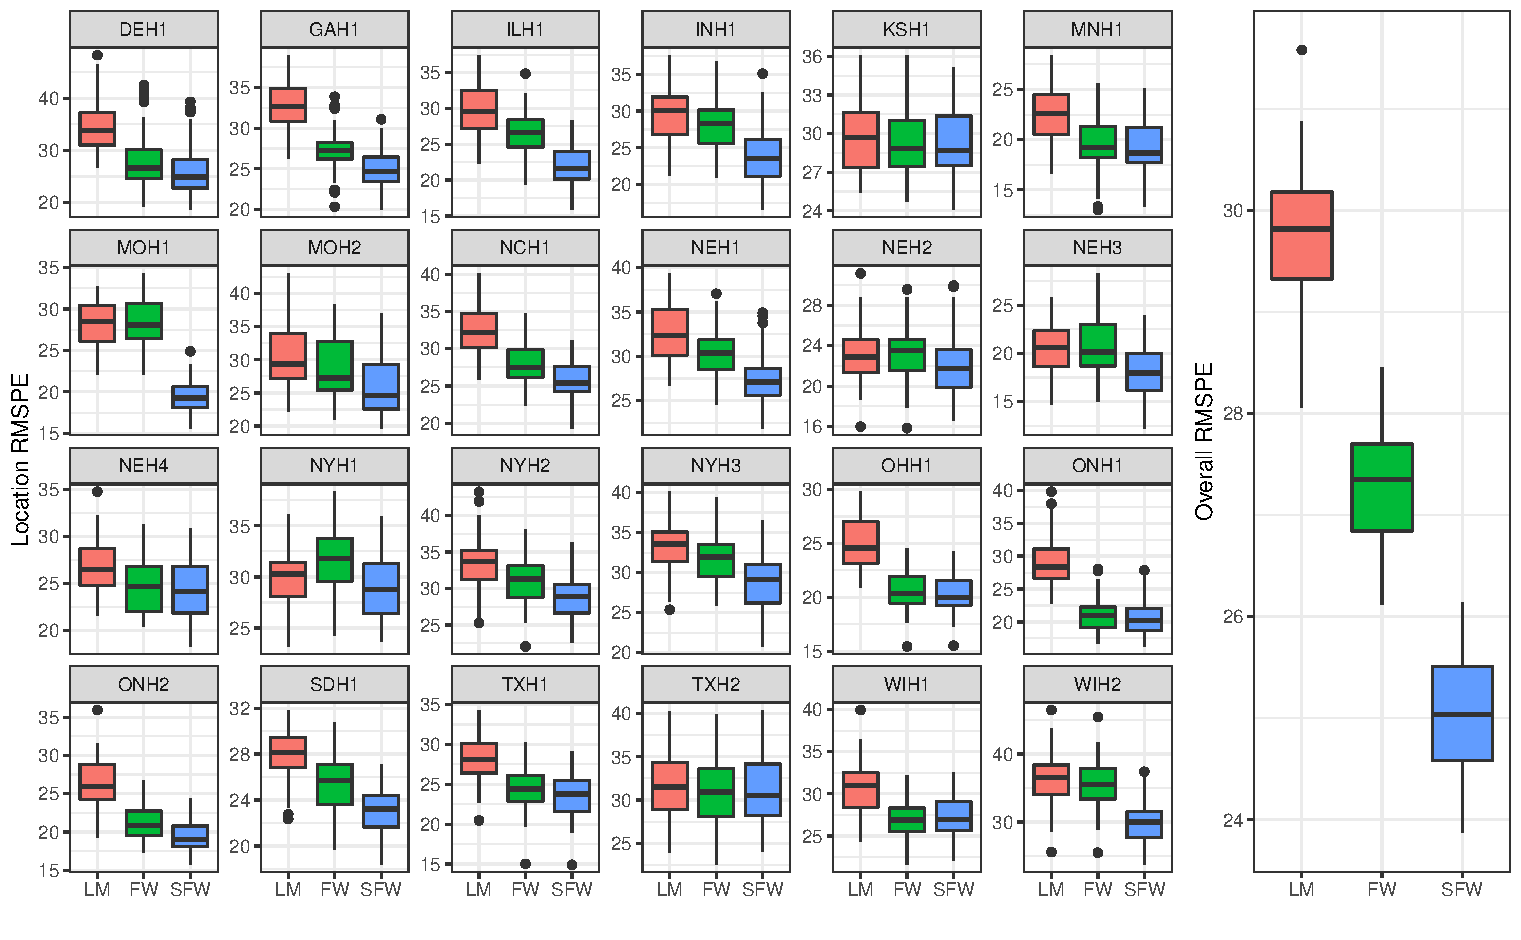
\includegraphics[width = 0.9\textwidth]{com_pred3.pdf}
	\end{figure}
\end{frame}



\begin{frame}
	\frametitle{Within-fields prediction}
Level of spatial correlation vs performance of SFW model.

	\begin{figure}[H]
		\centering
		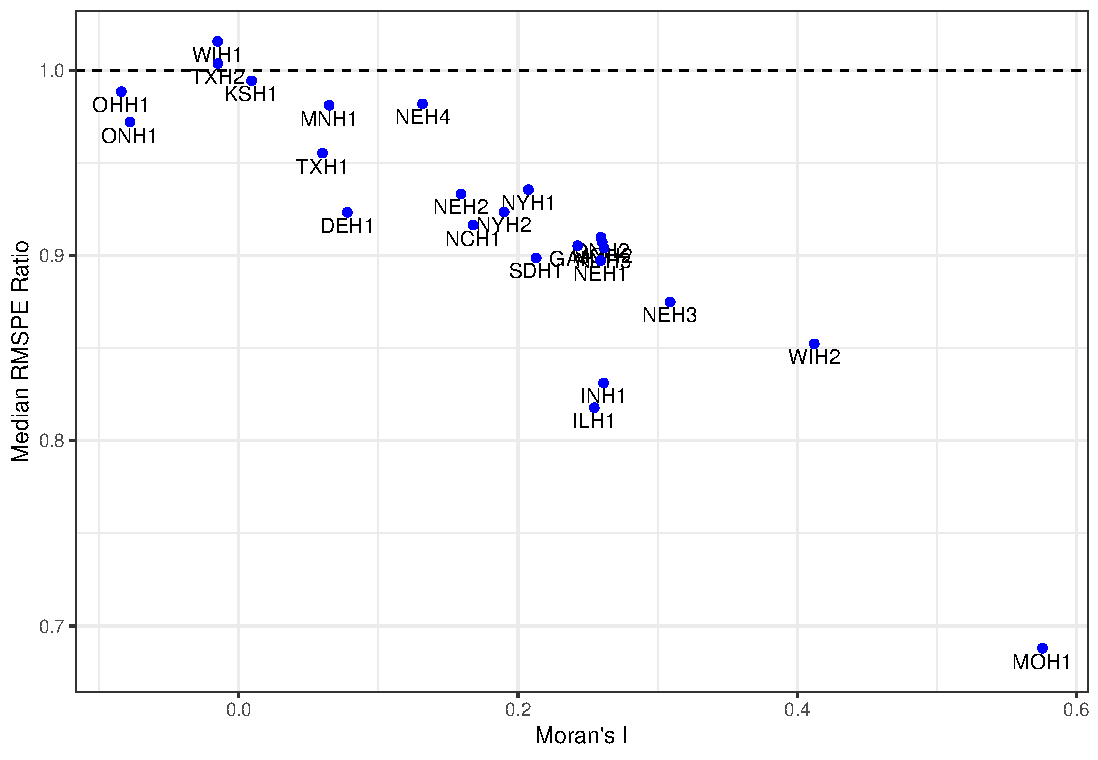
\includegraphics[width = 0.8\textwidth]{morans_i.pdf}
	\end{figure}
\end{frame}



\begin{frame}
	\frametitle{Out-of-fields prediction}
	
	\begin{itemize}
	\item Predict the grain yields in new fields.
	\item Need to learn how field effects depend on the weather and soil variables.
	\item More field trials and environmental data will lead to a more accurate and robust prediction.
	\end{itemize}
	
\end{frame}



\begin{frame}
	\frametitle{Out-of-fields prediction}
	Location-wise RMSPEs computed using temperature and rainfall data (x-axis), versus the location-wise RMSPEs computed not using any environment information (y-axis). 
	\begin{figure}[H]
		\centering
		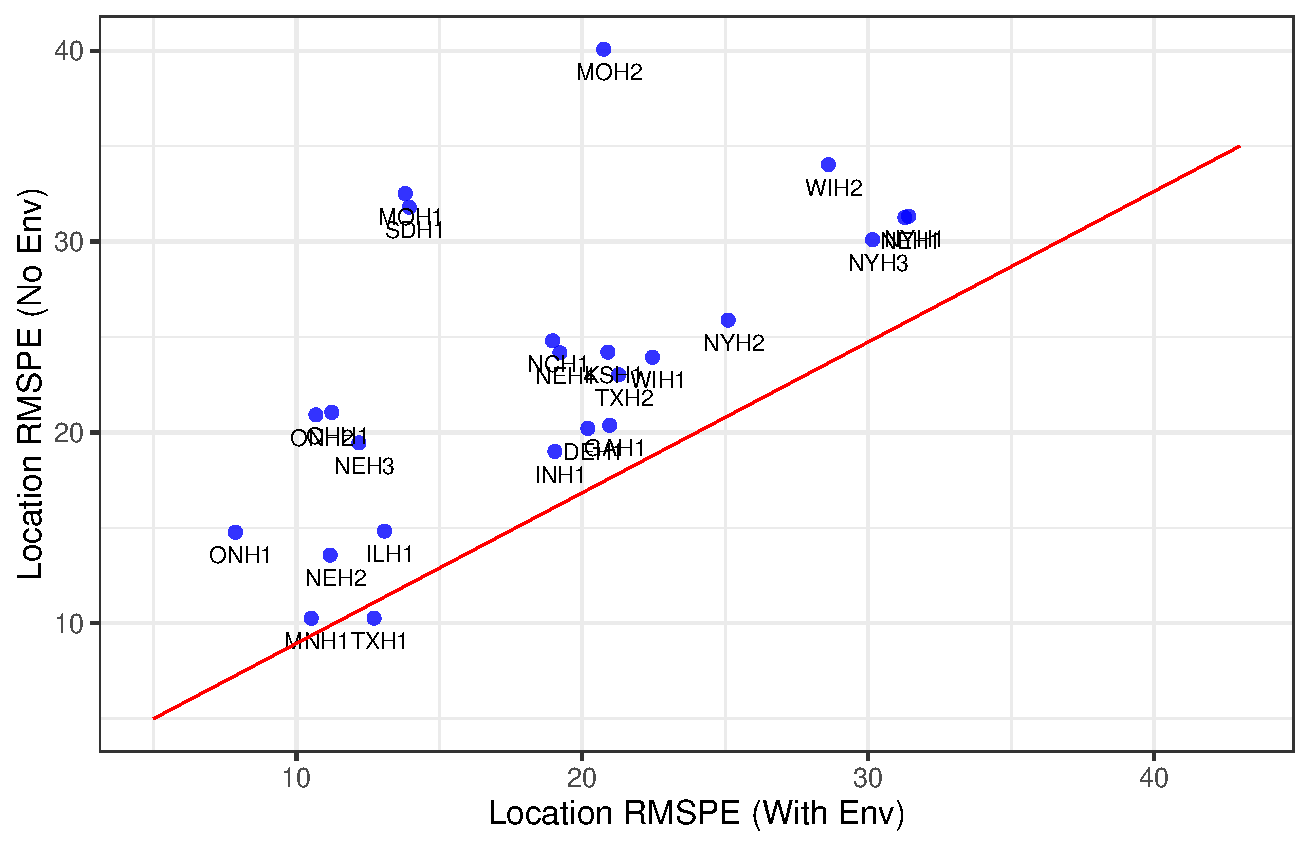
\includegraphics[width = 0.8\textwidth]{type3pred1.pdf}
	\end{figure}
	
\end{frame}


\begin{frame}
	\frametitle{Assessing Uncertainty about FW Regression Lines}

\begin{figure}[H]
  \begin{subfigure}{0.3\textwidth}
    \centering
    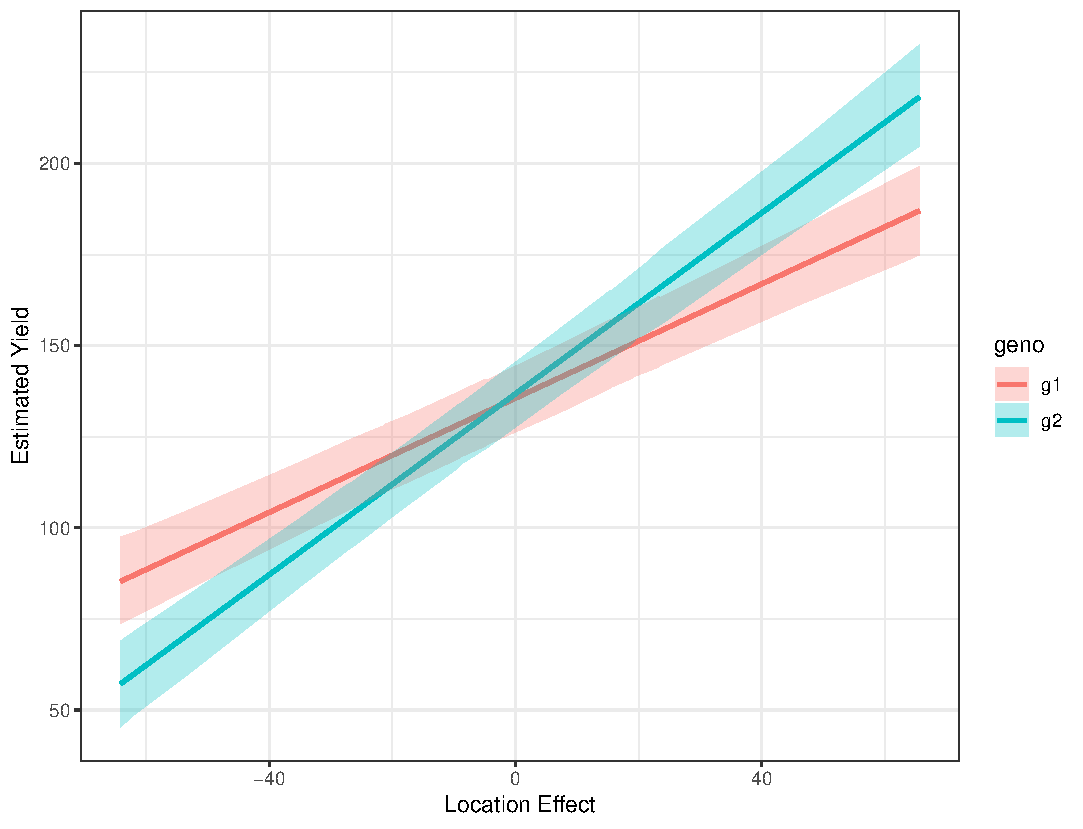
\includegraphics[width=.9\linewidth]{fwpair_1.pdf}
    \caption{}
  \end{subfigure}%
  \begin{subfigure}{0.3\textwidth}
    \centering
    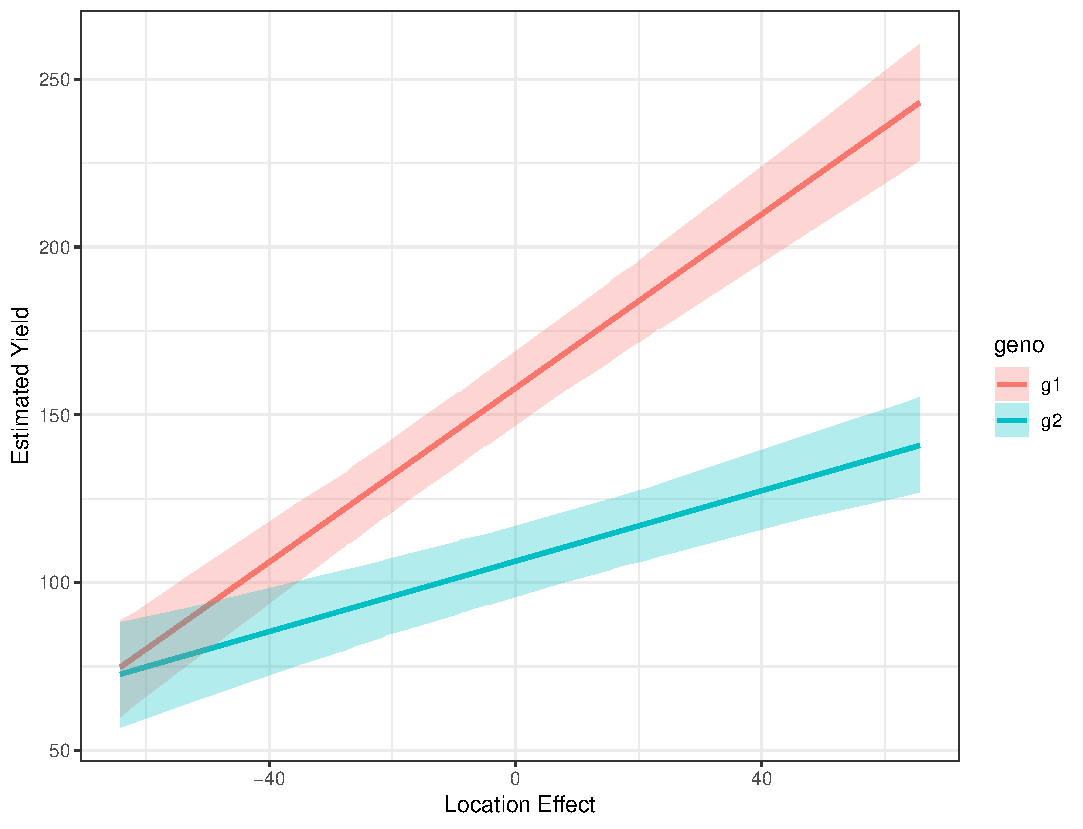
\includegraphics[width=.9\linewidth]{fwpair_2.pdf}
    \caption{}
  \end{subfigure}
  \begin{subfigure}{0.3\textwidth}\quad
    \centering
    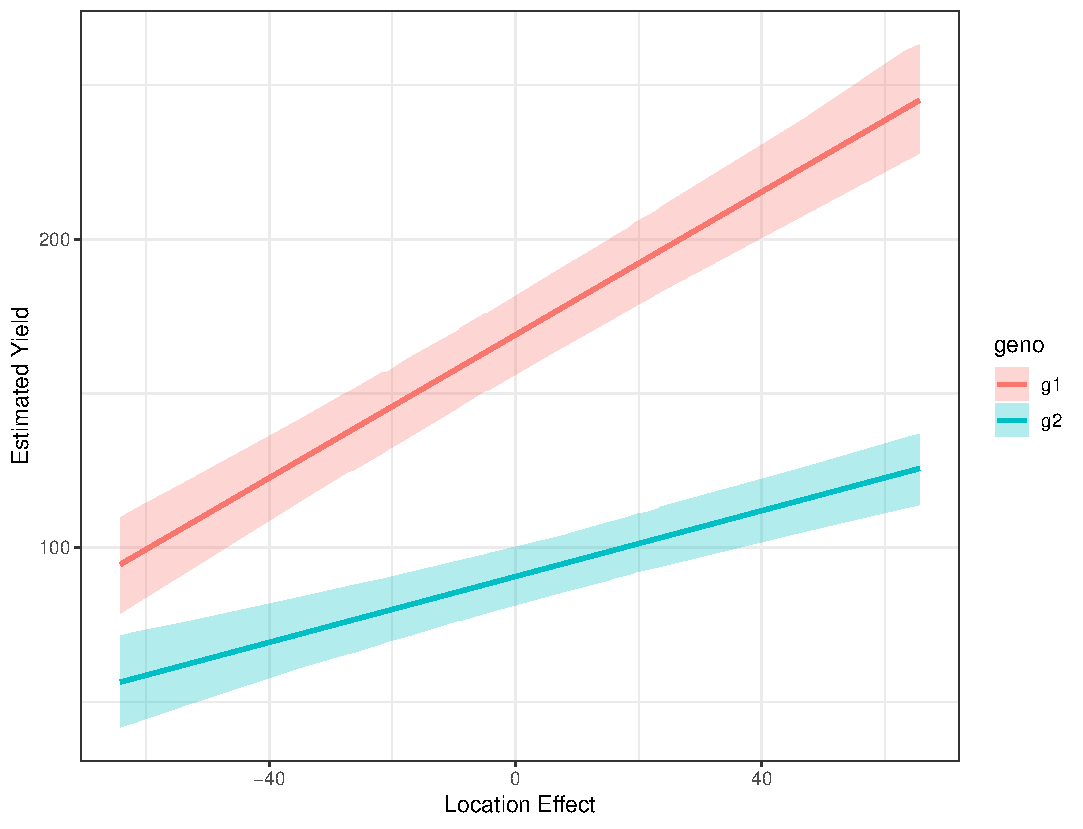
\includegraphics[width=.9\linewidth]{fwpair_3.pdf}
    \caption{}
  \end{subfigure}
  \medskip

  \begin{subfigure}{0.3\textwidth}
    \centering
    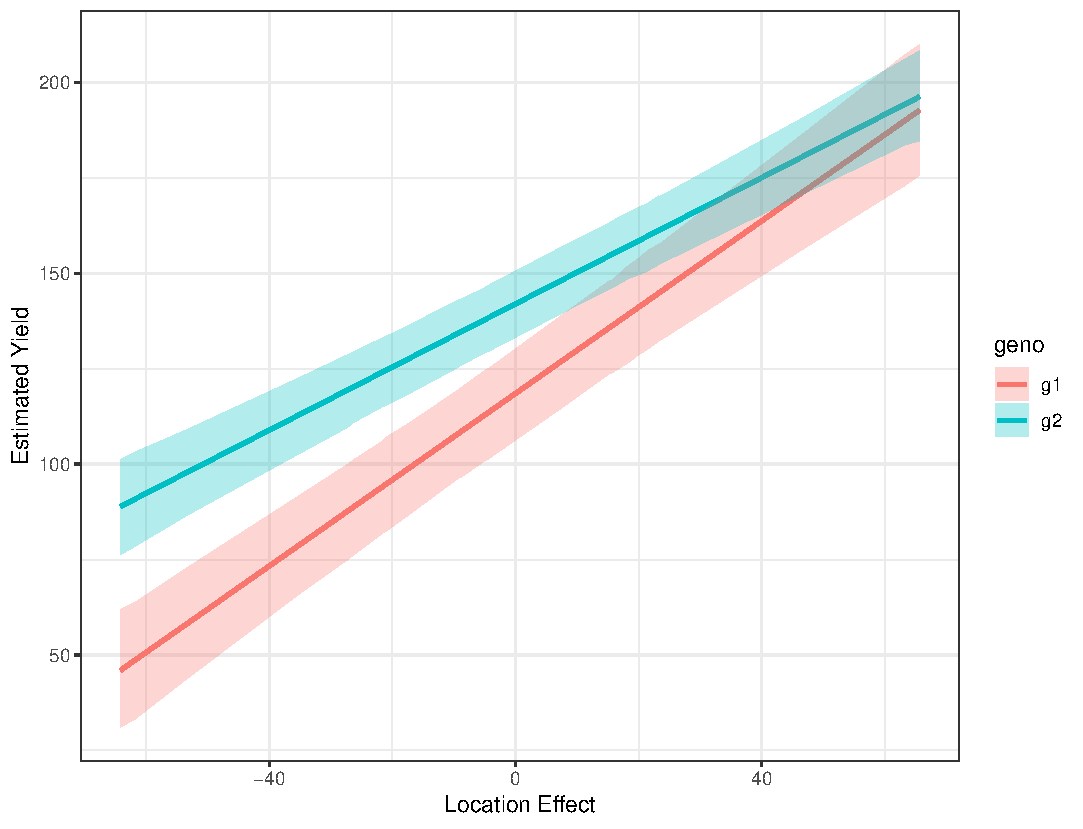
\includegraphics[width=.9\linewidth]{fwpair_4.pdf}
    \caption{}
  \end{subfigure}
  \begin{subfigure}{0.3\textwidth}
    \centering
    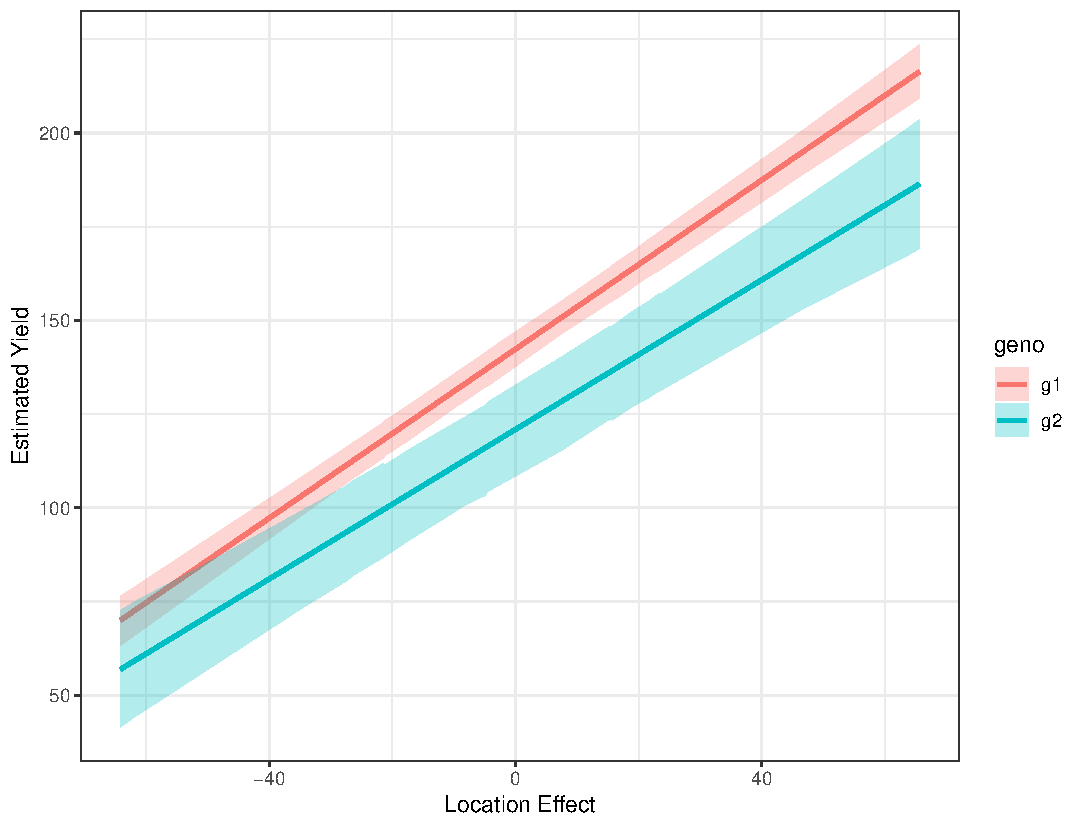
\includegraphics[width=.9\linewidth]{fwpair_5.pdf}
    \caption{}
  \end{subfigure}

  \caption{Estimated Yield vs Location Effect for pairs of genotypes}
\end{figure}


\end{frame}




\begin{frame}
\frametitle{References}
\bibliographystyle{apalike}
\bibliography{FWspatial}
\end{frame}


\begin{frame}%%     1
\begin{center}
\Huge Thank You!
\end{center}
\end{frame}















\end{document}



